\documentclass{elsarticle}

\title{?}
%\thanks{Research partially funded by projects EU 
% ASCENS (nr. 257414), EU QUANTICOL (nr. 600708), 
% IT MIUR CINA and PAR FAS 2007-2013 Regione Toscana TRACE-IT.}
% \thanks{An extended version containing full proofs is available at \cite{arxivCS}}
%}
%\author{Vincenzo Ciancia\inst{1} \and Matteo Sammartino\inst{2}}
%\institute{ISTI-CNR, Pisa \and Dipartimento di Informatica, Universit\`a di Pisa, Pisa }


\usepackage{amsmath}
\usepackage{amsthm}
\usepackage{amssymb}
\usepackage{subfigure}
\usepackage{tikz}
\usepackage{paralist}
\usepackage{aliascnt}
\usetikzlibrary{arrows,automata,positioning,calc,fit}
\newcommand{\subfigureautorefname}{\figureautorefname}
%\usepackage{cleveref}
\usepackage[hidelinks]{hyperref}
\newcommand{\cref}[1]{\autoref{#1}}
\usepackage{todonotes,mathpartir,enumerate,nicefrac}
\usepackage[all]{xy}
\usepackage[utf8]{inputenc}

\SelectTips{cm}{}

\DeclareMathOperator{\dom}{dom}

\newcommand{\todosm}[1]{\todo[size=\tiny]{#1}}

\newcommand{\autom}{A}
\newcommand{\hdma}{hDMA}
\newcommand{\hdmas}{\hdma s}

% Transition arrows
\newcommand{\Trarrow}{\Longrightarrow}
\newcommand{\Tr}[1]{\overset{#1}{\Trarrow}}
\newcommand{\TrP}[2]{\Tr{#1}_{#2}}
\newcommand{\htrind}[3]{\overset{#1}{\underset{#2}{\trarrow_{#3}}}}
\newcommand{\trind}[2]{\overset{#1}{\trarrow_{#2}}}

\newcommand{\pto}{\rightharpoonup}
\newcommand{\ul}[1]{{\underline{#1}}}
\newcommand{\restr}[2]{\ensuremath{\left.#1\right|_{#2}}}
\newcommand{\syncp}{\otimes}

\newcommand{\tstr}{\mathcal{T}}


% Symbols for ultimately periodic words
\newcommand{\regPerm}{I}
\newcommand{\regForg}{T}
\newcommand{\id}{\theta}
\newcommand{\forg}{\epsilon}
\newcommand{\ass}{\zeta}

\newcommand{\rrho}{\hat{\rho}}
\newcommand{\trho}{\tilde{\rho}}

\newcommand{\subs}[2]{\nicefrac{#1}{#2}}

\newcommand{\lab}[1]{{${\scriptstyle #1}$}}

%% Box
\newcommand{\tbox}[2]{
\medskip
\noindent%
\marginpar{#1}%
\fbox{%
\parbox{\linewidth}{#2}
}%
\medskip
}


\newcommand{\orb}{\mathit{orb}}

\newcommand{\trarrow}{\longrightarrow}
\newcommand{\tr}[1]{\overset{#1}{\trarrow}}

\newcommand{\weight}[1]{|#1|}
\newcommand{\acc}{\mathcal{A}}
\newcommand{\htr}[2]{\overset{#1}{\underset{#2}{\trarrow}}}
\newcommand{\inj}{\rightarrowtail}
\newcommand{\pinj}{\harpoon}
\newcommand{\names}{\mathcal{N}}
\newcommand{\Pow}{\mathcal{P}}

\newcommand{\confs}{\mathcal{C}}
\newcommand{\sub}[2]{[\nicefrac{#1}{#2}]}


\newcommand{\todocv}[1]{\todo[color=yellow,size=\tiny]{#1}}
\newcommand{\run}{r}
\newcommand{\Inf}{\mathit{Inf}}
\newcommand{\Lang}{\mathcal{L}}
\newcommand{\supp}{\mathit{supp}}
\newcommand{\Perm}{\mathbb{P}}
\renewcommand{\Im}{\mathit{Im}}


%% Theorems
%%% Fixes for autoref
\newtheorem{dummy}{***}[section] % add [section] for numbering within sections
\newcommand{\mynewtheorem}[2]{
  \newaliascnt{#1}{dummy}
  \newtheorem{#1}[#1]{#2}
  \aliascntresetthe{#1}
  % maybe we will squish some autoref defaults, but who cares?
  \expandafter\def\csname #1autorefname\endcsname{#2}
}


\newcommand{\theoremname}{Theorem}
\newcommand{\lemmaname}{Lemma}
\newcommand{\propositionname}{Proposition}
\newcommand{\definitionname}{Definition}
\newcommand{\examplename}{Example}
\newcommand{\remarkname}{Remark}
\newcommand{\propertyname}{Property}
\newcommand{\notationname}{Notation}
\newcommand{\conventionname}{Convention}

\theoremstyle{plain}
  \mynewtheorem{theorem}{Theorem}
  \mynewtheorem{proposition}{Proposition}
  \mynewtheorem{corollary}{Corollary}
  \mynewtheorem{property}{Property}
  \mynewtheorem{lemma}{Lemma}
  \mynewtheorem{conjecture}{Conjecture}
\theoremstyle{definition}
  \mynewtheorem{definition}{Definition}
  \mynewtheorem{example}{Example}
\theoremstyle{remark}
  \newtheorem*{notation}{\notationname}
  \mynewtheorem{remark}{Remark}
  \mynewtheorem{convention}{Convention}
  \mynewtheorem{invariant}{Invariant}


\raggedbottom
\frenchspacing

\begin{document}

 \begin{abstract}
Process calculi for service-oriented computing often feature generation of fresh resources. So-called nominal automata have been studied both as semantic models for such calculi, and as acceptors of languages of finite words over infinite alphabets. In this paper we investigate nominal automata that accept infinite words. These automata are a generalisation of deterministic Muller automata to the setting of nominal sets. We prove decidability of complement, union, intersection, emptiness and equivalence, and determinacy by ultimately periodic words. The key to obtain such results is to use finite representations of the (otherwise infinite-state) defined class of automata. The definition of such operations enables model checking of process calculi featuring infinite behaviours, and resource allocation, to be implemented using classical automata-theoretic methods.
\end{abstract}

\maketitle

\section{Introduction}\label{sec:introduction}%!TEX root=ndma.tex


This paper aims at contributing to the theory of formal verification of \emph{global computing} systems, by extending the theory of Muller automata to the case of infinite alphabets, while retaining decidability. In this way, it is possible to adapt the classical automata-theoretic approach to formal specification and verification \cite{ClarkeS01} to systems with resource generation capabilities, where the number of possible resources is infinite, provided that these systems enjoy a \emph{finite memory} property. 

Transition structures, in the form of automata, are used to represent logic formalisms interpreted over finite and infinite words, dating back to \cite{Buchi60,Elgot61}. The possibility of translating modal logic formulas to automata led to the development of \emph{model checking}. 
%
Systems that feature resource allocation (e.g.\ \cite{MilnerPW92}), typically in the form of \emph{name allocation}, pose specific challenges. For instance, they have ad-hoc notions of bisimulation, which cannot be captured by standard set-theoretic models. Transition structures that correctly model name allocation have been proposed in various forms, including coalgebras over presheaf categories \cite{FioreT01,BonchiBCG11,Miculan08,GhaniYV04,SammartinoM14}, history-dependent automata \cite{MontanariP05}, and automata over nominal sets \cite{BojanczykKL11}. Equivalence of these models has been established both at the level of base categories \cite{GadducciMM06,FioreS06,CianciaKM10} and of coalgebras \cite{CianciaM10}. More recently, the field of \emph{nominal automata} has essentially used the same structures, no longer as semantic models, but rather as acceptors of languages of finite words (see e.g., \cite{Tze11,KST12,GC11,BojanczykKL11}). In particular, the obtained languages are based on infinite alphabets, but still enjoy finite memory (in fact, the well known \emph{register automata} of Francez and Kaminski can be regarded as nominal automata, see \cite{BojanczykKL11}). 


The case of infinite words over nominal alphabets is more problematic, as an infinite word over an infinite alphabet is generally not \emph{finitely supported}.\footnote{The notion of finite support, coming from the theory of nominal sets, will be clarified later; roughly, finitely supported elements just use a finite set of names.} Consider a machine that reads any symbol from an infinite, countable alphabet, and never stores it. Clearly, such a machine has finite (empty) memory. The set of its traces is simply described as the set of all infinite words over the alphabet. However, in the language we have various species of words. Some of them are finitely supported, e.g.\ words that consist of the infinite repetition of a finite word. Some others are not finitely supported, such as the word enumerating all the symbols of the alphabet. Such words lay inherently out of the realm of nominal sets. However, the existence of these words does not give infinite memory to the language. More precisely, words without finite support can not be ``singled out'' by a finite memory machine; if a machine accepts one of them, then it will accept infinitely many others, including finitely supported words.  

This work aims at translating the above intuitions into precise mathematical terms, in order to define a class of languages made of infinite words over infinite alphabets, enjoying finite-memory properties. We extend automata over nominal sets to handle infinite words, by imposing a (Muller-style) acceptance condition 
over the \emph{orbits} (not the states!) of automata. By doing so, it turns out that our languages not only are finite-memory, but they retain computational properties, such as closure under boolean operations and decidability of emptiness (thus, containment and equivalence), which we prove by providing finite representations, and effective constructions. As in the case of standard $\omega$-automata, the shift to infinite words requires these results to be proved from scratch, as it is not possible to merely extend proofs from the finite words case. These results enable automata-theoretic model checking to be performed on systems with infinite resources, using traditional model-checking algorithms. 

Furthermore, we prove that the defined languages are determined by their ultimately-periodic fragments. This theorem is fundamental for \emph{learning} logical properties (see e.g., \cite{MP95}, or \cite{FCCTW08}) and has been used to provide a complete minimisation procedure for equivalent representations of Muller automata \cite{CV12}. Establishing this theoretical result in the nominal case is an important step towards the application of such techniques to global computing scenarios.

\section{Example: peer-to-peer system}\label{sec:example}
%!TEX root=ndma.tex

In order to introduce the presented topic, in this section we discuss an application of nominal automata to distributed systems. Consider an idealized \emph{peer-to-peer} system where each peer receives queries from an arbitrary, unbounded number of other peers, represented by an infinite set of unique identifiers. Each peer buffers requests in a finite queue. Then one query is selected, among the buffered ones, and is served by establishing a temporary connection with the target. Peers are not normally supposed to terminate, thus their relevant properties ought to predicate on infinite words. On the other hand, actions executed by peers carry information about other peers, which are drawn from an infinite set, therefore the symbols constituting words are infinite. Finally, each peer has finite memory. This is the key to maintain decidability, and is mathematically modeled by the notion of \emph{finite support} in nominal automata. Once established that our languages are made of infinite words over an infinite alphabet, but retain a finite memory property, we can use automata to characterize properties of local peers in a global environment. 
%
We assume three kinds of observable actions for peers: arrival of a new query from $p$, written $q(p)$; selection of a query to serve and connection to its sender $p$, written $s(p)$; disconnection from $p$, written $d(p)$.


Variants of a communication protocol in this setting may have very different behaviors. Policies characterizing desired ones, for instance fairness requirements, can be specified by automata. For decidability reasons, policies should be \emph{deterministic}: they should always consider all possible actions from a given state, even if not all of them will be accepted, and each action should have a unique outcome. 
%
Our main example will be the specification of a ``first come first serve'' peer selection policy for queries, named \emph{FCFS fair policy}; we shall also discuss a policy that takes into account a number of locally identified ``friend peers'' taking priority over the others, that we call \emph{friend policy}. 

\emph{FCFS fair policy.}
We model query selection by a \emph{fair} FCFS discipline: queries from already buffered peers are discarded. We assume that the buffer has size $n$. 
%
%
\begin{figure}[t]
\centering
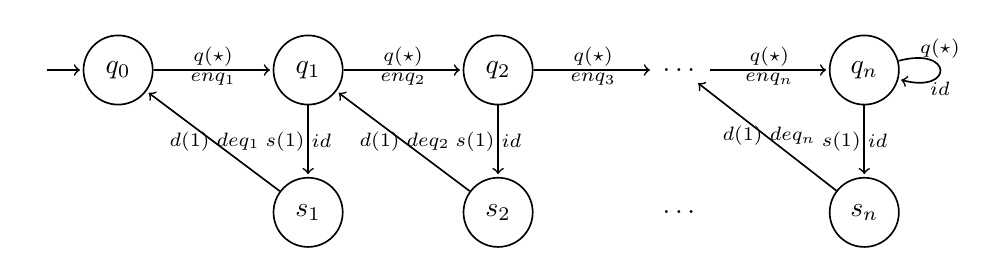
\begin{tikzpicture}[->,shorten >=1pt,auto,node distance=2.8cm,semithick,initial text={},scale=1, every node/.style={scale=1}]

  \node[state,initial] (q0) {$q_0$}; 
  \node[state,right=10ex of q0] (q1) {$q_1$};
  \node[state,right=10ex of q1] (q2) {$q_2$};
  \node[right=10ex of q2] (dots) {$\dots$};
  \node[state,right=10ex of dots] (qn) {$q_n$};

  \node[state,below=6ex of q1] (s1) {$s_1$};
  \node[state,below=6ex of q2] (s2) {$s_2$};
  \node[below=10ex of dots] (dotss) {$\dots$};
  \node[state,below=6ex of qn] (sn) {$s_n$};


  \path (q0) edge node[inner sep=1pt,above] {\lab{q(\star)}} node[inner sep=1pt,below] {\lab{enq_1}} (q1);
  \path (q1) edge node[inner sep=1pt,above] {\lab{q(\star)}} node[inner sep=1pt,below] {\lab{enq_2}} (q2);
  \path (q2) edge node[inner sep=1pt,above] {\lab{q(\star)}} node[inner sep=1pt,below] {\lab{enq_3}}  (dots);
  \path (dots) edge node[inner sep=1pt,above] {\lab{q(\star)}} node[inner sep=1pt,below] {\lab{enq_n}} (qn);

  \path (q1) edge node[inner sep=1pt,left] {\lab{s(1)}} node[inner sep=1pt,right] {\lab{id}} (s1);
  \path (q2) edge node[inner sep=1pt,left] {\lab{s(1)}} node[inner sep=1pt,right] {\lab{id}} (s2);
  \path (qn) edge node[inner sep=1pt,left] {\lab{s(1)}} node[inner sep=1pt,right] {\lab{id}} (sn);
  \path (qn) edge[loop right] node[inner sep=4pt,above] {\lab{q(\star)}} node[inner sep=4pt,below] {\lab{id}} (qn);

  \path (s1) edge node[inner sep=1pt,left] {\lab{d(1)}} node[inner sep=1pt,right] {\lab{deq_1}} (q0);
  \path (s2) edge node[inner sep=1pt,left] {\lab{d(1)}} node[inner sep=1pt,right] {\lab{deq_2}} (q1);
  \path (sn) edge node[inner sep=1pt,left] {\lab{d(1)}} node[inner sep=1pt,right] {\lab{deq_n}} (dots);


\end{tikzpicture}
\caption{Automaton for the FCFS policy.}
\label{fig:fcfs}
\vskip -10pt
\end{figure}
%
The automaton is shown in \autoref{fig:fcfs}. Each state $q_i,s_i$ is equipped with $i$ registers, for $i=1,\dots,n$, and $q_0$ has no registers. Registers can store identifiers, and are local to states (we will discuss this aspect throughout the paper), thus each transition is equipped with a function expressing how registers in the target state take values from those of the source state. We have two such functions: $enq_i(x)$, mapping $i$ to $\star$ and $x < i$ to $x$, and $deq_i$, mapping $x$ to $x+1$.
%
The intuition is that transitions from $q_i$ to $q_{i+1}$ labeled with $\star$ correspond to buffering a ``fresh'' query, from a peer whose identiy is not already known, and thus it is stored in register $i+1$. The loop on $q_n$ discards new peers when the buffer is full. The transition from $q_i$ to $s_i$ picks the query $p$ from register $1$, that is always the oldest one, and establishes a connection to $p$; the transition from $s_i$ to $q_{i-1}$ removes $p$ from the buffer, and shifts the registers' content so that register $1$ contains the query that arrived right after the one of $p$. Our automaton should (1) be deterministic and (2) have a Muller-style accepting condition. For (1), we assume each state has all possible outgoing transitions: those not shown in \autoref{fig:fcfs} are assumed to go to a sink state. For (2), we take all subsets of the states, excluding the sink one, as Muller sets; that is: behaviors that go through states and transitions depicted in \autoref{fig:fcfs} are all accepted. 

\emph{Friend queries.} A \emph{friend query} is a query coming from a ``friend'' peer, which should be served as soon as possible, that is: after the current query has been served. To model such scenarios, one can introduce an action $q_f(p)$ to model a friend query from $p$. An automaton that correctly handles such queries can be obtained from the one of \autoref{fig:fcfs} as follows: we add a transition from $q_i$ to $q_{i+1}$, for each $i=0,\dots,n-1$, labelled with $q_f(\star)$ and with the map $top_i$, sending $1$ to $\star$ and $x > 1$ to $x-1$; furthermore, a looping transition on $q_n$ is added with label $q_f(\star)$ and map $id$, which discards friend queries when the buffer is full. Intuitively, $top_i$ always stores the friend query in register $1$, so that transitions $s(1)$ will always pick it, and shifts the priority of all the other peers.

\section{Background}\label{sec:background}%!TEX root=ndma.tex
\paragraph{Notation.} 
Throughout the paper: $f \colon X \to Y$ is a total function, $f \colon X \inj Y$ is total and injective, $f \colon X \pto Y$ is partial; $\dom(f)$ is the subset of $X$ where $f$ is defined, $\Im(f)$ its image. Symbol $\omega$ denotes the set of natural numbers. For $s$ a sequence, we let $s_i$ or $s(i)$ denote its $i^{\mathit{th}}$ element. $R^*$ is the symmetric, transitive, reflexive closure of binary relation $R$. We use $\circ$ for (partial) function composition and also for ``relational'' composition, as usual, by seeing functions as relations.

We shall now briefly introduce nominal sets; we refer the reader to \cite{GP02} for more details on the subject. We assume a countable set of \emph{names} $\names$, and we write $\Perm$ for the group of finite-kernel permutations of $\names$, namely those bijections $\pi \colon \names \to \names$ such that the set $\{ a \mid \pi(a) \neq a \}$ is finite.
\begin{definition}
A \emph{nominal set} is a set $X$ along with an action for $\Perm$, that is a function $\cdot \colon \Perm \times X \to X$ such that, for all $x \in X$ and $\pi,\pi' \in \Perm$, $id_\names \cdot x = x$ and $(\pi \circ \pi') \cdot x = \pi \cdot (\pi' \cdot x)$. Also, it is required that each $x \in X$ has \emph{finite support}, meaning that there exists a finite $S \subseteq \names$ such that, for all $\pi \in \Perm$, $\restr{\pi}{S} = id_S$ implies $\pi \cdot x = x$. We denote the least\footnote{It is a theorem that whenever there is a finite support, there is also a least support.} such $S$ with $\supp(x)$. An \emph{equivariant function} from nominal set $X$ to nominal set $Y$ is a function $f : X \to Y$ such that, for all $\pi$ and $x$, $f(\pi \cdot x) = \pi \cdot f(x)$.
\end{definition}
%
\begin{definition}
Given $x \in X$, the \emph{orbit} of $x$, denoted by $\orb(x) $, is the set $\{ \pi \cdot x \mid \pi \in \Perm\} \subseteq X$. For $S \subseteq X$, we write $\orb(S)$ for $\{ \orb(x) \mid x \in S\}$. We call $X$ \emph{orbit-finite} when $\orb(X)$ is finite.
\end{definition}

\noindent Note that $\orb(X)$ is a partition of $X$. The prototypical nominal set is $\names$ with $\pi \cdot a = \pi(a)$ for each $a \in \names$; we have $\supp(a) = \{a\}$, and $\orb(a) = \names$.


\section{Nominal \texorpdfstring{$\omega$}{omega}-regular languages}\label{sec:languages}%!TEX root=ndma.tex

In the following, we extend \emph{Muller automata} to the case of nominal alphabets. Traditionally, automata can be deterministic or non-deterministic. In the case of finite words, non-deterministic nominal automata are not closed under complementation, whereas the deterministic ones are; similar considerations apply to the infinite words case. Thus, we adopt the deterministic setting in order to retain complementation.

\begin{definition}\label{def:ndma}
 A \emph{nominal deterministic Muller automaton} (nDMA) is a tuple $(Q,\tr{},q_0,\acc)$ where:
 
  \begin{itemize}
  \item $Q$ is an orbit-finite nominal set of \emph{states}, with $q_0 \in Q$ the \emph{initial state};
  
  \item $\acc \subseteq \Pow(\orb(Q))$ is a set of sets of orbits, intended to be used as an acceptance condition in the style of Muller automata.
  
  \item $\htr{}{}$ is the \emph{transition relation}, made up of triples $q_1 \tr{a} q_2$, having \emph{source} $q_1$, \emph{target} $q_2$, \emph{label} $a \in \names$;
  
  \item the transition relation is \emph{deterministic}, that is, for each $q \in Q$ and $a \in \names$ there is exactly one transition with source $q$ and label $a$;
  
  \item the transition relation is \emph{equivariant}, that is, invariant under permutation: there is a transition $q_1 \tr a q_2$ if and only if, for all $\pi$, also the transition $\pi \cdot q_1 \tr{\pi(a)} \pi \cdot q_2$ is present.
 \end{itemize}
\end{definition}
%
In nominal sets terminology, the transition relation is an \emph{equivariant function} of type $Q \times \names \to Q$.  Notice that nDMA are infinite state, infinitely branching machines, even if orbit finite. For effective constructions we employ equivalent finite structures (see Section \ref{sec:hd-automata}). Definition \ref{def:ndma} induces a simple definition of acceptance, very close to the classical one. In the following, fix a nDMA $A=(Q,\tr{},q_0,\acc)$.

\begin{definition}
\label{def:inf-word}
 An infinite \emph{word} $\alpha \in \names^\omega$ is an infinite sequence of symbols in $\names$. Words have \emph{point-wise} permutation action, namely $(\pi \cdot \alpha)_i = \pi(\alpha_i)$, making a word finitely supported if and only if it contains finitely many different symbols. 
\end{definition}

\begin{definition}\label{def:nominal-run}
 Given a word $\alpha \in \names^\omega$, a \emph{run} of $\alpha$ from $q \in Q$ is a sequence of states $\run \in Q^\omega$, such that $\run_0 = q$, and for all $i$ we have $\run_i \tr{\alpha_i} \run_{i+1}$. 
 By determinism (see Definition \ref{def:ndma}), for each infinite word $\alpha$, and each state $q$, there is exactly one run of $\alpha$ from $q$, that we call $\run^{\alpha,q}$, or simply $\run^{\alpha}$ when $q=q_0$.
\end{definition}

\begin{definition}\label{def:inf-set}
 For $\run \in Q^\omega$, let $\Inf(\run)$ be the set of \emph{orbits} that $\run$ traverses infinitely often, i.e., $\orb(q) \in \Inf(\run)$ iff. for all $i$, there is $j > i$ s.t. $\run_j \in \orb(q)$.
\end{definition}

\begin{definition}
 A word $\alpha$ is \emph{accepted} by state $q$ whenever $\Inf(\run^{\alpha,q}) \in \acc$. We let $\Lang_{A,q}$ be the set of all accepted words by $q$ in $A$; we omit $A$ when clear from the context, and $q$ when it is $q_0$, thus $\Lang_A$ is the language of the automaton $A$. We say that $\Lang \subseteq \names^\omega$ is a \emph{nominal $\omega$-regular language} if it is accepted by a nDMA.
\end{definition}

\begin{remark}\label{rem:simple-alphabet} We use $\names$ as alphabet. One can chose any orbit-finite nominal set; the definitions of automata and acceptance are unchanged, and finite representations are similar. Using $\names$ simplifies the presentation, especially in Section \ref{sec:hd-automata}.
\end{remark}

\begin{example}\label{exa:session}
 Consider the nDMA in \cref{fig:example-session}. We have $Q = \{q_0\} \cup \{q_a \mid a \in \names\}$. For all $\pi$, we let $\pi \cdot q_0 = q_0$, $\pi \cdot q_a = q_{\pi(a)}$. We have $\supp(q_0) = \emptyset$, and $\supp(q_a) = \{ a \}$. For all $a$, let $q_0 \tr{a} q_a$, $q_a \tr{a} q_0$, and for $b \neq a$, $q_a \tr b q_a$. Each of the infinite ``legs'' of the automaton rooted in $q_0$ remembers a different name, and returns to $q_0$ when the same name is encountered again. There are two orbits, namely $\orb_0 = \{ q_0 \}$ and $\orb_1 = \{ q_a \mid a \in \names \}$. We let $\acc = \{ \{ \orb_0, \orb_1 \} \}$. For acceptance, a word needs to cross both orbits infinitely often. Thus, $\Lang_{q_0}=\{aua \mid a \in \names, u \in (\names\setminus\{a\})^* \}^\omega$.
% 
This is an idealized version of a service, where each in a number of potentially infinite users (represented by names) may access the service, reference other users, and later leave. Infinitely often, an arbitrary symbol occurs, representing an ``access''; the next occurrence of the same symbol denotes a ``leave''. One could use an  alphabet with two infinite orbits to distinguish the two kinds of action (see Remark \ref{rem:simple-alphabet}), or reserve two distinguished names of $\names$ to be used as ``brackets'' before the different occurrences of other names, adding more states.
\end{example}

\begin{figure}[t]
\vskip -10pt
\subfigure[]{
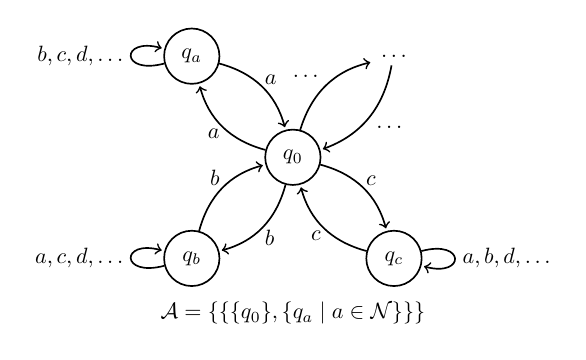
\begin{tikzpicture}[->,shorten >=1pt,auto,node distance=15ex,semithick,initial text={},scale=0.8, every node/.style={scale=0.8}]  
  \node[state] (q0)               {$q_0$};
  \node[state] (qa) [above left of = q0] {$q_a$};
  \node[state] (qb) [below left of = q0] {$q_b$};
  \node[state] (qc) [below right of = q0] {$q_c$};
  \node (qany) [above right of = q0] {$\ldots$};
  	\coordinate (Middle) at ($(qb)!0.5!(qc)$);
  \node (acc) [below=3ex of Middle] {$\acc = \{ \{ \{ q_0 \} , \{ q_a \mid a \in \names \}\}\}$};
% 
%  
  \path (q0) edge [bend left]  node[inner sep=1pt] {$a$} (qa);
  \path (q0) edge [bend left]  node[inner sep=1pt] {$b$} (qb);
  \path (q0) edge [bend left]  node[inner sep=1pt] {$c$} (qc);
  \path (q0) edge [bend left]  node {$\ldots$} (qany);  
  \path (qa) edge [bend left]  node[inner sep=1pt] {$a$} (q0)
             edge [loop left] node {$b,c,d,\ldots$} (qa);  
  \path (qb) edge [bend left]  node[inner sep=1pt] {$b$} (q0)
             edge [loop left] node {$a,c,d,\ldots$} (qb);  
  \path (qc) edge [bend left]  node[inner sep=1pt] {$c$} (q0)
             edge [loop right] node {$a,b,d,\ldots$} (qc);  
  \path (qany) edge [bend left]  node {$\ldots$} (q0);
             edge [loop right] node {} (qany);
%
\end{tikzpicture}
\label{fig:example-session}
}
\hspace{2ex}
\subfigure[]{
{\centering
 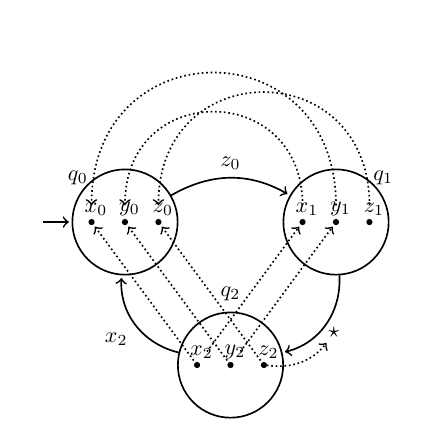
\begin{tikzpicture}[->,shorten >=1pt,auto,node distance=2.8cm,semithick,initial text={},scale=0.8, every node/.style={scale=0.8}] 
\tikzstyle{every state}=[minimum size=10ex]
  \tikzstyle{register}=	[circle,fill,draw,inner sep=0pt,minimum size=2pt]
%	
%
\node[register,label={[shift={(2pt,-2pt)}]above:$x_0$}] (reg00) {};
  \node[register,label={[shift={(2pt,-2pt)}]above:$y_0$}] (reg01) [right=10pt of reg00] {};
  \node[register,label={[shift={(2pt,-2pt)}]above:$z_0$}] (reg02) [right=10pt of reg01] {};
  \node[register,label={[shift={(2pt,-2pt)}]above:$x_1$}] (reg10) [right=50pt of reg02] {};
  \node[register,label={[shift={(2pt,-2pt)}]above:$y_1$}] (reg11) [right=10pt of reg10] {};
  \node[register,label={[shift={(2pt,-2pt)}]above:$z_1$}] (reg12) [right=10pt of reg11] {};
  \node[register,label={[shift={(2pt,-2pt)}]above:$y_2$}] (reg21) at ($(reg02)!0.5!(reg10)$) [yshift=-15ex] {};
  \node[register,label={[shift={(2pt,-2pt)}]above:$x_2$}] (reg20) [left=10pt of reg21] {};
  \node[register,label={[shift={(2pt,-2pt)}]above:$z_2$}] (reg22) [right=10pt of reg21] {};
  \node[state,initial,fit={(reg00) (reg01) (reg02)},inner sep=2ex] (q0) {};
  \node[above left=-1ex of q0] (lab0) {$q_0$}; 
  \node[state,fit={(reg10) (reg11) (reg12)},inner sep=2ex] (q1) {};
  \node[above right=-1ex of q1] (lab1) {$q_1$}; 
  \node[state,fit={(reg20) (reg21) (reg22)},inner sep=2ex] (q2) {};
  \node[above=1pt of q2] (lab2) {$q_2$}; 

  \path (q0) edge [bend left] node {$z_0$} (q1);
  \path (q1) edge [bend left=40]  node[inner sep=1pt] (star) {$\star$} (q2);
  \path (q2) edge [bend left=40] node {$x_2$} (q0);	
  \path (reg10) edge[densely dotted,out=90,in=90,looseness=2,shorten >=5pt,shorten <=5pt] (reg01);
  \path (reg11) edge[densely dotted,out=90,in=90,looseness=2,shorten >=5pt,shorten <=5pt] (reg00);
  \path (reg12) edge[densely dotted,out=90,in=90,looseness=2,shorten >=5pt,shorten <=5pt] (reg02);
  \path (reg20) edge[densely dotted,shorten <=5pt] (reg10);
  \path (reg21) edge[densely dotted,shorten <=5pt] (reg11);
  \path (reg22) edge[bend right,densely dotted] (star);
  \path (reg20) edge[densely dotted,shorten <=1pt] (reg00);
  \path (reg21) edge[densely dotted,shorten <=1pt] (reg01);
  \path (reg22) edge[densely dotted,shorten <=1pt] (reg02);
\end{tikzpicture}
}
\label{fig:upwords-ex}
}

\vspace{-4ex}
\subfigure[]{
{
\centering
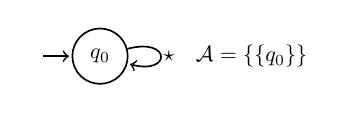
\begin{tikzpicture}[->,shorten >=1pt,auto,node distance=2.8cm,semithick,initial text={},scale=0.8, every node/.style={scale=0.8}]
%
%	
  \node[state,initial] (q0) {$q_0$}; 
  \node[right=5ex of q0] {$\acc = \{ \{ q_0 \} \}$};
%
  \path (q0) edge [loop right]  node[inner sep=1pt] (star) {$\star$} (q0);
\end{tikzpicture}
}
\label{fig:hd-names-omega}
}
%
\hspace{10ex}
\subfigure[]{
{\centering
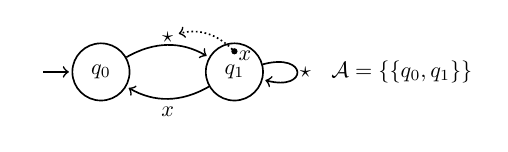
\begin{tikzpicture}[->,shorten >=1pt,node distance=14ex,auto,semithick,initial text={},scale=0.8, every node/.style={scale=0.8}]
  \tikzstyle{every state}=[minimum size=6ex]
  \tikzstyle{register}=	[circle,fill,draw,inner sep=0pt,minimum size=2pt]	
  \node[state,initial] (q0) {$q_0$}; 
  \node[state,right of=q0] (q1) {};  
  \node (lab1) at (q1) {$q_1$};  \node[register,label={[xshift=-3pt,yshift=-2pt]right:$x$}] (reg) [above=1pt of lab1] {};
  \node[right=5ex of q1] {$\acc = \{\{q_0,q_1\}\}$};
  \path (q0) edge [bend left]  node[inner sep=1pt] (star) {$\star$} (q1);
  \path (q1) edge[loop right] node[inner sep=1pt] {$\star$} (q1);
  \path (q1) edge [bend left] node {$x$} (q0);
  \path (reg) edge[densely dotted,bend right] (star);
\end{tikzpicture}
}
\label{fig:hd-of-example}
}
\label{fig:automata}
\vskip -10pt
\caption{Some automata, together with their accepting conditions.
}\vskip-10pt
\end{figure}

\noindent Accepted words may fail to be finitely supported. However, languages are. This adheres to the intuition that a machine running forever may read an unbounded amount of different pieces of data, but still have finite memory.

\begin{theorem}\label{thm:languages-finitely-supported}
 For $\Lang$ a language, and $\pi\in \Perm$, let $\pi\cdot \Lang = \{\pi \cdot \alpha \mid \alpha \in \Lang\}$. For each state $q$ of an nDMA, $\Lang_{q}$ is finitely supported.
\end{theorem}


\section{Finite automata}\label{sec:hd-automata}
%!TEX root=ndma.tex

In this section, we introduce finite representations of nDMAs. These are similar to classical finite-state automata, but each state is equipped with local registers. There is a notion of assignment to registers, and it is possible to accept, and eventually store, \emph{fresh} symbols. Technically, these structures extend \emph{history-dependent automata} (see \cite{Pistore99}), introducing acceptance of infinite words.

\begin{definition}\label{def:hdma}
 A \emph{history-dependent deterministic Muller automaton} (\hdma) is a tuple $(Q,\weight -,q_0,\rho_0,\htr{}{},\acc)$
 where: 
 \begin{itemize}
  \item \vskip -6pt $Q$ is a finite set of \emph{states};
  \item for $q \in Q$, $\weight{q}$ is a finite set of \emph{local names} (or \emph{registers}) of state $q$;
  \item $q_0 \in Q$ is the \emph{initial state};
  \item $\rho_0 : \weight{q_0} \inj \names$ is the \emph{initial assignment};
  \item $\acc \subseteq \Pow(Q)$ is the \emph{accepting condition}, in the style of \emph{Muller automata};
  \item $\htr{}{}$ is the \emph{transition relation}, made up of quadruples $q_1 \htr{l}{\sigma} q_2$, having \emph{source} $q_1$, \emph{target} $q_2$, label $l \in \weight{q_1} \uplus \{\star\}$, and \emph{history} $\sigma : \weight{q_2} \inj \weight{q_1} \cup \{l\}$;
  \item the transition relation is \emph{deterministic} in the following sense: for each $q_1 \in Q$,   there is exactly one transition with source $q_1$ and label $\star$, and exactly one transition with source $q_1$ and label $x$ for each $x \in \weight{q_1}$.
 \end{itemize}
\end{definition}
%

\begin{remark}
To keep the notation lightweight, we do not use a \emph{symmetry} attached to states of an \hdma. It is well known (see \cite{MontanariP05}) that symmetries are needed for existence of canonical representatives; we consider this aspect out of the scope of this work. Note that (classical) Muller automata do not have canonical representatives up-to language equivalence. To obtain those, one can use two-sorted structures as in \cite{CV12}. Even though this idea could be applied to hDMAs, this is not straightforward, and requires further investigation.
\label{rem:no-symmetry}
\end{remark}
%
In the following we fix an \hdma{} $A = (Q,\weight -,q_0,\rho_0,\htr{}{},\acc)$. We overload notation (e.g., for the inf-set of a word) from \cref{sec:languages}, as it will be always clear from the context whether we are referring to an nDMA or to an \hdma. Acceptance of $\alpha \in \names^\omega$ is defined using the \emph{configuration graph} of $A$.

\begin{definition}\label{def:configuration}
 The set $\confs(A)$ of \emph{configurations} of $A$ consists of the pairs $(q,\rho)$ such that $q \in Q$ and $\rho : \weight q \inj \names$ is an injective \emph{assignment} of names to registers.
\end{definition}

\begin{definition}
\label{def:configuration-graph}
The \emph{configuration graph} of $A$ is a graph with edges of the form  
$(q_1,\rho_1) \tr a (q_2,\rho_2)$ where the source and destination are configurations, and $a \in \names$. There is one such edge iff there is a transition $q_1 \htr l \sigma q_2$ in $A$ and either $l \in \weight{q_1}$, $\rho_1(l) = a$, and $\rho_2 = \rho_1 \circ \sigma$, or $l = \star$, $a \notin \Im(\rho_1)$, $\rho_2 = (\rho_1 \circ \sigma)\sub{a}{\sigma^{-1}(\star)}$.
\end{definition}
% 
%
The definition deserves some explanation. Fix a configuration $(q_1,\rho_1)$. Say that name $a\in \names$ is \emph{assigned to} the register $x \in \weight{q_1}$ if $\rho_1(x) = a$. When $a$ is not assigned to any register, it is \emph{fresh} for a given configuration. Then the transition $q_1 \htr l \sigma q_2$, under the assignment $\rho_1$, consumes a symbol as follows: either $l \in \weight{q_1}$ and $a$ is the name assigned to register $l$, or $l$ is $\star$ and $a$ is fresh. The destination assignment $\rho_2$ is defined using $\sigma$ as a binding between local registers of $q_2$ and local registers of $q_1$, therefore composing $\sigma$ with $\rho_1$ and eventually adding a freshly received name, whenever $\star$ is in the image of $\sigma$. For readability, we assume that the functional update $\sub{a}{\sigma^{-1}(\star)}$ is void when $\star \notin \Im(\sigma)$. The following lemma clarifies the notion of determinism that we use.

\begin{lemma}
\label{lem:deterministic-configuration-graph}
 For each configuration $(q_1,\rho_1)$ and symbol $a \in \names$, there is exactly one configuration $(q_2,\rho_2)$ such that $(q_1,\rho_1) \tr a (q_2,\rho_2)$.
\end{lemma}
%
We use the notation $(q_1,\rho_1) \Tr{v} (q_2,\rho_2)$ to denote a path that spells $v$ in the configuration graph. Furthermore, we define runs of infinite words.
%

\begin{definition}
 A \emph{run} $\run$ of an infinite word $\alpha \in \names^\omega$ from configuration $(q,\rho)$ is a sequence $(q_i,\rho_i)$ of configurations, indexed by $\omega$, such that $(q_0,\rho_0)=(q,\rho)$ and for all $i$, in the configuration graph, we have $(q_i,\rho_i) \tr{\alpha_i} (q_{i+1},\rho_{i+1})$. 
\end{definition}
%
Finally, after a simple corollary of  \cref{lem:deterministic-configuration-graph}, we define acceptance of \hdmas. 
%
\begin{proposition}
\label{prop:unique-path}
Given $(q_1,\rho_1) \in \confs(A)$ and $v \in \names^\omega$, there exists a unique path $(q_1,\rho_1) \Tr{v} (q_2,\rho_2)$ in the configuration graph of $A$. Similarly, for each word $\alpha$ and configuration $(q,\rho)$, there is a unique run $\run^{\alpha,q,\rho}$ from $(q,\rho)$. We omit $q$ and $\rho$ from the notation, when dealing with the \emph{initial configuration} $(q_0,\rho_0)$.
\end{proposition}
%
\begin{definition}\label{def:acceptance-of-hdmas}
 Consider the unique run $\run$ of an infinite word $\alpha$ from configuration $(q,\rho)$. 
 Let $\Inf(\run)$ denote the set  of states that appear infinitely often in the first component of $\run$. By finiteness of $Q$, $\Inf(\run)$ is not empty. The automaton $A$ accepts $\alpha$ whenever $\Inf(r) \in \acc$. In this case, we speak of the \emph{language} $\Lang_A$ of words accepted by the automaton.
\end{definition}
%
As an example, the language $\names^\omega$ of all infinite words over $\names$ is recognised by the \hdma{} in \cref{fig:hd-names-omega}; the initial assignment $\rho_0$ is necessarily empty, and so is the history $\sigma$ along the transition.
%
%
Differently from nDMAs, \hdmas\ have finite states. Finite representations are useful for effective operations on languages, as we shall see later. The similarity between configuration graphs of \hdmas, and nDMAs, is deep and is the essence of the proof of \autoref{pro:nset-to-nom-and-back} below. These are similar to the categorical equivalence results in \cite{GadducciMM06,FioreS06}; however, notice that representing infinite branching systems using  ``allocating transitions'' requires further machinery, similar to what is studied in \cite{CianciaM10}.
%
\begin{proposition}\label{pro:nset-to-nom-and-back}
 For each (orbit-finite) nDMA there is a finite hDMA accepting the same language, and vice versa.
\end{proposition}
%
\begin{example}
Consider the \hdma\ in \autoref{fig:hd-of-example},
%
where the labelled dot within $q_1$ represents its register, and the dashed line depicts the history from $q_1$ to $q_0$ (we omit empty histories). This automaton accepts the language of \cref{exa:session}. In fact, $q_0$ is the only element in the orbit of the initial state of the nDMA, and $q_1$ canonically represents all $q_a$, $a \in \names$. This notation for \hdmas{} will be used throughout the paper.
\end{example}


\section{Synchronized product and boolean operations}\label{sec:sync-product}
%!TEX root=ndma.tex
\newcommand{\eq}[1]{#1}
\newcommand{\syncQ}{Q_{\syncp}}
\newcommand{\syncW}[1]{\weight{#1}_{\syncp}}
\newcommand{\syncAss}{\rho_0^{\syncp}}
\newcommand{\syncInit}{q_0^{\syncp}}
\newcommand{\syncTr}[1]{\xymatrix@C-=4ex{\ar[r]^{#1}&\!_{\syncp}}}
\newcommand{\syncHtr}[2]{\xymatrix@C-=4ex{\ar[r]^{#1}_{#2}&\!_{\syncp}}}
\newcommand{\regrule}{\textsc{(Reg)}}
\newcommand{\allrule}{\textsc{(Alloc)}}
\newcommand{\cproj}{\pi}

The product of two finite automata uses the well-known \emph{synchronized product} construction. In this section we define this operation on the underlying \emph{transition structures} of \hdmas{}, i.e.\ on tuples $\tstr = (Q,\weight{-},q_0,\rho_0,\trarrow)$ (we want to be parametric w.r.t.\ the accepting condition). One should  be careful in handling registers. When forming pairs of states, some of these registers could be constrained to have the same value. Thus, states have the form $(q_1,q_2,R)$, where $R$ is a relation linking registers of $q_1$ and $q_2$ that represent the same register in the synchronized product. This is implemented by quotienting registers w.r.t.\ the equivalence $R^*$ induced by $R$; the construction is similar to the case of register automata, and to the construction of products in named sets given in \cite{CianciaM10}.

Given two transition structures $\tstr_i = (Q_i,\weight{-}_i,q_0^i,\rho_0^i,\trarrow_i)$, $i=1,2$, we define their synchronized product $\tstr_1 \syncp \tstr_2$. Given $q_1 \in Q_1$,$q_2 \in Q_2$, $Reg(q_1,q_2)$ is the set of relations that are allowed to appear in states of the form $(q_1,q_2,R)$, namely those $R \subseteq \weight{q_1}_1 \times \weight{q_2}_2$ such that, for each $(x,y) \in R$, there is no other $(x',y') \in R$ with $x'=x$ or $y'=y$. This avoids inconsistent states where the individual assignment for $q_1$ or $q_2$ would not be injective. In the following we assume $[x]_{R^*}$ (the canonical representative of the equivalence class of $x$ in $R^*$) to be $\{x\}$ when $x$ does not appear in any pair of $R$.


\begin{definition}
\label{def:syncp}
$\tstr_1 \syncp \tstr_2$ is the tuple $(\syncQ,\syncW{-},\syncInit,\syncAss,\syncTr{\quad})$ where:
\begin{itemize}
	\item 
	$\syncQ := \{ (q_1,q_2,R) \mid q_1 \in Q_1,q_2 \in Q_2,R \in Reg(q_1,q_2)\}$;
	%
	\item $\syncW{(q_1,q_2,R)} := (\weight{q_1}_1 \cup \weight{q_2}_2)_{/R^*}$, for $(q_1,q_2,R) \in \syncQ$;
	%
	\item $\syncInit := (q_0^1,q_0^2,R_0)$, where $R_0:= \{ (x_1,x_2) \in \weight{q_0^1}_1 \times \weight{q_0^2}_2 \mid \rho_0^1(x_1) = \rho_0^2(x_2) \}$;
	%
	\item $\rho_0([x]_{R_0^*}) = \rho_0^i (x)$ whenever $x \in \weight{q_0^i}_i$, $i \in \{1,2\}$; 
	%
	\item transitions are generated by the following rules
\end{itemize}
	%
		\begin{mathpar}
			\inferrule[(Reg)]
			{ q_1 \htrind{l_1}{\sigma_1}{1} q_1' \\
			q_2 \htrind{l_2}{\sigma_2}{2} q_2' 
			\\\\
			\exists i \in \{1,2\} : l_i \in \names \land [l_i]_{R^*} = \{l_1,l_2\} \cap \names}
			{ (q_1,q_2,R) \syncHtr{[l_i]_{R^*}}{\sigma_R}
			(q_1',q_2',S) } 
			%}
			\quad\;
			\inferrule[(Alloc)]
			{ q_1 \htrind{l_1}{\sigma_1}{1} q_1' \quad q_2 \htrind{l_2}{\sigma_2}{2} q_2' \quad l_1,l_2 = \star} 
			{ (q_1,q_2,R) \syncHtr{\star}{\sigma_A} (q_1',q_2',S) }
		\end{mathpar}
	where $S := \sigma_2^{-1} \circ R \cup \{(l_1,l_2)\} \circ \sigma_1 $ and
	\begin{align*}
		\sigma_\tau([x]_{S^*}) &:= 
		\begin{cases}
			[\sigma_i(x)]_{R^*} & x \in \weight{q'_i}_i \land \sigma_i(x) \neq \star \\
			[l_{3-i}]_{R^*} & x \in \weight{q'_i}_i \land \sigma_i(x) = \star \land \tau = R \\
			\star & x \in \weight{q'_i}_i \land \sigma_i(x) = \star \land \tau = A
		\end{cases}
	\end{align*}
\end{definition}
%
 Before explaining in detail the formal definition, we remark that the relation $S$ is well defined, i.e.\ it belongs to $Reg(q_1',q_2')$: the addition of $\{(l_1,l_2)\}$ to $R$ is harmless, as will be explained in the following, and $\sigma_1$ and $\sigma^{-1}_2$ can never map the same value to two different values (as they are functions) or vice versa (as they are injective).
%
The definition of $\syncInit$ motivates the presence of relations in states: $R_0$-related registers are the ones that are assigned the same value by $\rho_0^1$ and $\rho_0^2$; these form the same register of $\syncInit$, so $\syncAss$ is well-defined. The synchronization mechanism is implemented by rules \regrule{} and \allrule{}: they compute transitions of $(q_1,q_2,R) \in \syncQ$ from those of $q_1$ and $q_2$ as follows.

Rule \regrule{} handles two cases. First, if the transitions of $q_1$ and $q_2$ are both labelled by registers, say $l_1$ and $l_2$, and these registers correspond to the same one in $(q_1,q_2,R)$ (condition $[l_i]_{R^*} = \{l_1,l_2\}$, recalling that $[l_i]_{R^*}$ cannot contain more labels due to injectivity of register maps), then \regrule{} infers a transition labelled with $[l_i]_{R^*}$ (the specific $i$ is not relevant). The target state of this transition is made of those of the transitions from $q_1$ and $q_2$, plus a relation $S$ obtained by translating $R$-related registers to $S$-related registers via $\sigma_1$ and $\sigma_2$. In this case, adding the pair $(l_1,l_2)$ to $R$ in the definition of $S$ has no effect, as it is already in $R$. The inferred history $\sigma_R$ just combines $\sigma_1$ and $\sigma_2$, consistently with $S^*$.

The other case for \regrule{} is when a fresh name is consumed from just one state, e.g.\ $q_2$.
This name must coincide with the value assigned to the register $l_1$ labelling the transition of $q_1$. Therefore the inferred label is $[l_1]_{R^*}$. The target relation $S$ changes slightly. Suppose there are $l'_1 \in \weight{q'_1}$ and $l'_2\in \weight{q'_2}$ such that $\sigma_1(l'_1) = l_1$ and $\sigma_2(l'_2) = \star$; after $q_1$ and $q_2$ perform their transitions, both these registers are assigned the same value, so we require $(l'_1,l'_2) \in S$. This pair is forced to be in $S$ by adding $(l_1,\star)$ to $R$ when computing $S$. This does not harm well-definedness of $S$, because $[l_1]_{R^*}$ is a singleton (rule premise $[l_1]_{R^*} = \{l_1,\star\} \cap 	\names = \{l_1\}$), so no additional, inconsistent identifications are added to $S^*$ due to transitivity. If either $l_1$ or $\star$ is not in the image of the corresponding history map, then augmenting $R$ has no effect, as the relational composition discards $(l_1,\star)$. The history $\sigma_R$ should map $[l_2']_{S^*}$ to $[l_1]_{R^*}$: this is treated by the second case of its definition; all the other values are mapped as before.

Transitions of $q_1$ and $q_2$ consuming a fresh name on both sides are turned by \allrule{} into a unique transition with freshness: $S$ is computed by adding $(\star,\star)$ to $R$, thus the registers to which the fresh name is assigned (if any) form one register in the overall state; the inferred history $\sigma_A$ gives the freshness status to this register, and acts as usual on other registers.

\begin{remark}
\label{rem:syncp-fin-det}
$\tstr_1 \syncp \tstr_2$ is finite-state and deterministic. In fact, every set in the definition of $\syncQ$ is finite. As for determinism, given $(q_1,q_2,R) \in \syncQ$, each $l \in \syncW{(q_1,q_2,R)} \cup \{\star\}$ uniquely determines which labels $l_1$ and $l_2$ should appear in the rule premises (e.g. if $l = \{l_1\}$, with $l_1 \in \weight{q_1}_1$, then $l_2 = \star$), and by determinism each $q_i$ can do a unique transition labeled by $l_i$.
\end{remark}
%
We shall now relate the configuration graphs of $\tstr_1 \syncp \tstr_2$, $\tstr_1$ and $\tstr_2$.
%
\begin{definition}
Let $((q_1,q_2,R),\rho) \in \confs(\tstr_1 \syncp \tstr_2)$. Its $i$-th projection, denoted $\cproj_i$, is defined as
$\cproj_i((q_1,q_2,R),\rho) = (q_i,\rho_i)$ with $\rho_i := \lambda x \in \weight{q_i}_i.\rho([x]_{R^*})$
\end{definition}
%
Projections always produce valid configurations in $\confs(\tstr_1)$ and $\confs(\tstr_2)$: injectivity of $\rho_i$ follows from the definition of $Reg(q_1,q_2)$, ensuring that two different $x_1,x_2 \in \weight{q_i}_i$ cannot belong to the same equivalence class of $R^*$, i.e.\ cannot have the same image through $\rho_i$. The correspondence between edges is formalized as follows.

\begin{proposition}
\label{prop:edges-correspondence}
Given $C \in \confs(\tstr_1 \syncp \tstr_2)$: 
\begin{inparaenum}[(i)]
	if $C \tr{a} C'$ then $\cproj_i(C) \tr{a} \cproj_i(C')$, $i = 1,2$;
	\label{sync-to-each}
	\item if $\cproj_i(C) \trind{a}{i} C_i$, $i=1,2$, 
	then $\exists C' : C\tr{a} C'$ and $\cproj_i(C) = C_i$.
	\label{each-to-sync}
\end{inparaenum}
\end{proposition}
%
\begin{corollary}
\label{cor:paths-correspondence}
Let $C_0 = (\syncInit,\rho_0)$. We have a path $C_0 \tr{a_0} \dots \tr{a_{n-1}} C_n$ in the configuration graph of $\tstr_1 \syncp \tstr_2$ if and only if we have paths $\cproj_i(C_0) \tr{a_0} \dots \tr{a_{n-1}} \cproj_i(C_n)$ in the configuration graphs of $\tstr_i$, for $i=1,2$. The correspondence clearly holds also for infinite paths, i.e.\ runs.
\end{corollary}
%
This result allows us to relate the $\Inf$ of runs in the defined transition structures.
%
\begin{theorem}
\label{thm:inf-correspondence}
Given $\alpha \in \names^\omega$, let $r$ be a run for $\alpha$ in the configuration graph of $\tstr_1 \syncp \tstr_2$, and let $r_1$ and $r_2$ be the corresponding runs for $\tstr_1$ and $\tstr_2$, according to \cref{cor:paths-correspondence}. Then $\pi_1(Inf(r)) = Inf(r_1)$ and $\pi_2(Inf(r)) = Inf(r_2)$.
\end{theorem}
%
%!TEX root=ndma.tex
\newcommand{\compl}[1]{\overline{#1}}
%
Let $\Lang_1$ and $\Lang_2$ be $\omega$-regular nominal languages, and let $\autom_1 = (\tstr_1,\acc_1)$  and $\autom_2 = (\tstr_2,\acc_2)$ be automata for these languages, where $\tstr_1$ and $\tstr_2$ are the underlying transition structures. By \cref{thm:inf-correspondence} above, 
we are now able to show that constructing the automaton for a boolean combination of $\Lang_1$ and $\Lang_2$ amounts to defining an appropriate accepting set for $\tstr_1 \syncp \tstr_2$.


\begin{theorem}
Using the transition structure $\tstr_1 \syncp \tstr_2$, define the accepting conditions $\acc_\cap = \{ S \subseteq \syncQ \mid \pi_1(S) \in \acc_1 \land \pi_2(S) \in \acc_2 \}$, $\acc_\cup = \{ S \subseteq \syncQ \mid \pi_1(S) \in \acc_1 \lor \pi_2(S) \in \acc_2 \} $ and $\acc_{\compl{\Lang_1}} = \Pow(Q_1) \setminus \acc_1$, where $Q_1$ are the states of $\autom_1$. The obtained \hdma{}s accept, respectively, $\Lang_1 \cap \Lang_2$, $\Lang_1 \cup \Lang_2$, and $\compl{\Lang_1}$.
\label{thm:bool-closure}
\end{theorem}
%
\begin{theorem}
\label{thm:decidable}
Emptiness and, as a corollary, equality of $\omega$-regular nominal languages are decidable.
\end{theorem}


\section{Ultimately-periodic words}\label{sec:up-words}%!TEX root=ndma.tex
%
%
%
An \emph{ultimately periodic} word is a word of the form $uv^\omega$, with $u,v$ finite words. Given a language of infinite words $\Lang$, let $UP(\Lang)$ be its \emph{ultimately periodic fragment} $\{ \alpha \in \Lang \mid \alpha = uv^\omega \land u,v \; \text{are finite} \}$. It has been proven in \cite{CalbrixNP93,Buchi62} that, for every two $\omega$-regular languages $\Lang_1$ and $\Lang_2$, $UP(\Lang_1) = UP(\Lang_2)$ implies $\Lang_1 = \Lang_2$, i.e.\ $\omega$-regular languages are characterised by their ultimately periodic fragments.
In this section we aim to extend this result to the nominal setting. 

The preliminary result to establish, as in the classical case, is that every non-empty nominal $\omega$-regular language $\Lang$ contains at least one ultimately periodic word. For $\omega$-regular languages, this involves finding a loop through accepting states in the automaton and iterating it. For \hdmas, freshness constraints could forbid consuming the same name in consecutive traversals of the same transition.
We first show that, given a loop in a \hdma{}, there always is a path induced by consecutive traversals of the loop, such that its initial and final configurations coincide. Thus, such path can be taken an arbitrary number of times.

Fix a loop $L \;:=\; p_0 \htr{l_0}{\sigma_0} p_1 \htr{l_1}{\sigma_1} \dots \htr{l_{n-1}}{\sigma_{n-1}} p_0$ (the specific \hdma{} is not relevant). We write $\ul{i}$ for $i \mod n$. For all $i=0,\dots,n-1$, let $\widehat{\sigma}_i \colon \weight{p_\ul{i+1}} \pto \weight{p_i}$ be the partial maps telling the history of old registers and ignoring the new ones, formally $\widehat{\sigma}_i := \sigma_i \setminus \{ (x,y) \in \sigma_i \mid y = \star \}$, and let $\widehat{\sigma} \colon \weight{p_0} \pto \weight{p_0}$ be their composition $\widehat{\sigma}_0 \circ \widehat{\sigma}_1 \dots \circ \widehat{\sigma}_{n-1}$. We define the set $I$ as the greatest subset of $\dom(\widehat{\sigma})$ such that $ \widehat{\sigma}(I) = I$,
i.e.\ $I$ are the registers of $p_0$ that ``survive'' along $L$. We denote by $T$ all the other registers, namely $T := \weight{p_0} \setminus I$. These are registers whose content is eventually discarded (not necessarily within a single loop traversal), as the following lemma states.
%
%
\begin{lemma}
\label{lem:rho-forget}
Given any $x \in T$, let $\{x_j\}_{j \in J_x}$ be the smallest sequence that satisfies the following conditions: $x_0 = x$ and $x_{j+1} = \sigma_{\ul{j}}^{-1}(x_j)$, where $j+1 \in J_x$ only if $\sigma_{\ul{j}}^{-1}(x_j)$ is defined. Then $J_x$ has finite cardinality.
\end{lemma}
%
Now, consider any assignment $\rrho_0 \colon \weight{p_0} \to \names$. We give some lemmata about paths that start from $(p_0,\rrho_0)$ and are induced by consecutive traversals of $L$. The first one says that the assignment for $I$ given by $\rrho_0$ is always recovered after a fixed number of traversals of $L$, regardless of which symbols are consumed. In the following, given a sequence of transitions $P$, we write $(q_1,\rho_1) \TrP{v}{P} (q_2,\rho_2)$ whenever $(q_1,\rho_1) \Tr{v} (q_2,\rho_2)$ and such path is induced by $P$.
%
\begin{lemma} 
\label{lem:idI}
There is $\id \geq 1$ such that, for all $v_0,\dots,v_{\id-1}$ satisfying $(p_0,\rrho_0) \TrP{v_0}{L} (p_0,\rrho_1) \TrP{v_1}{L} \dots \TrP{v_{\id-1}}{L} (p_0,\rrho_\id)$ we have $\restr{ \rrho_\id }{I} = \restr{ \rrho_0 }{I}$.
\end{lemma}
%
The second one says that, after a minimum number of traversals of $L$, a configuration can be reached where the initial values of $T$, namely those assigned by $\rrho_0$, cannot be found in any of the registers.
%
\begin{lemma}
There is $\forg \geq 1$ s.t., for all $\gamma \geq \forg$ ,there are $v_0,\dots,v_{\gamma-1}$ satisfying $(p_0,\rrho_0) \TrP{v_0}{L} (p_0,\rrho_1) \TrP{v_1}{L} \dots \TrP{v_{\gamma-1}}{L} (p_0,\rrho_\gamma)$, with $\Im(\rrho_\gamma) \cap \rrho_0(T) = \varnothing$.
\label{lem:forgetT}
\end{lemma}
%
%
We give the dual of the previous lemma: if we start from a configuration where registers are not assigned values in $\rrho_0(T)$, then these values can be assigned back to $T$ in a fixed number of traversals of $L$, regardless of the initial assignment.

\begin{lemma}
There is $\ass \geq 1$ such that,
for any $\trho_0 \colon \weight{p_0} \to \names$ with $\Im(\trho_0) \cap \rrho_0(T) = \varnothing$, there are $v_0,\dots,v_{\ass-1}$ satisfying $ (p_0,\trho_0) \TrP{v_0}{L} (p_0,\trho_1) \TrP{v_1}{L} \dots \TrP{v_{\ass-1}}{L} (p_0,\trho_\ass)$, with $\restr{\trho_\ass}{T} = \restr{\rrho_0}{T}$.
\label{lem:initT}
\end{lemma}
%
%
Finally, we combine the above lemmata. We construct a path where: (1) the values assigned to $T$ are forgotten and then recovered (2) the values assigned to $I$ are swapped, but the initial assignment is periodically regained. Therefore, the length of such path should allow (1) and (2) to ``synchronize'', so that the final assignment is again $\rrho_0$.

\begin{theorem}
\label{thm:loop}
%
For each loop $L$ with initial state $p_0$, and assignment $\rrho_0 \colon \weight{p_0} \to \names$, there are $v_0,\dots,v_n$ such that $(p_0, \rrho_0) \TrP{v_0}{L} (p_0, \rrho_1) \TrP{v_1}{L} \cdots \TrP{v_n}{L} (p_0,\rrho_0) $.
\end{theorem}
%
\begin{example} We justify the construction on the \hdma{} of \cref{fig:upwords-ex}, with initial assignment $\rho_0(x_0) = a$,$\rho_0(y_0) = b$ and $\rho_0(z_0) = c$. Consider the loop $L$ formed by all the depicted transitions. We have $I = \{x_0,y_0\}$ and $T = \{z_0\}$. Look at the path $(q_0,[\subs{a}{x_0},\subs{b}{y_0},\subs{c}{z_0}]) \tr{c} (q_1,[\subs{b}{x_1},\subs{a}{y_1},\subs{c}{z_1}]) \tr{d} (q_2,[\subs{b}{x_2},\subs{a}{y_2},\subs{d}{z_2}])
	\tr{b} (q_0,[\subs{b}{x_0},\subs{a}{y_0},\subs{d}{z_0}])$ where $d \neq a,b,c$. The values of $x_0$ and $y_0$ are swapped according to the permutation $(a \; b)$, and $d$ is assigned to $z_0$. Our aim is to recover $\rho_0$ again. According to \cref{lem:idI}, $x_0$ and $y_0$ get their assignment back in $\theta = 2$ traversals of $L$ (in fact $(a\; b)^2 = (a\; b)$). As for $z_0$, its assignment is established in the second transition, but $c$ should not have been assigned to any register of $q_1$ in order for it to be consumed during this transition. This is where \cref{lem:forgetT} comes into play: it says that in at least $\epsilon = 1$ traversals of $L$ the name $c$ is discarded. This is exactly what happens in the path shown above. Then we can assign $c$ to $z_0$ in another $\zeta = 1$ traversal of $L$, according to \cref{lem:initT}. Since $\epsilon + \zeta  = \theta = 2$, traversing $L$ twice is enough (e.g., consider the path $cdbdca$).
\end{example}
%
\noindent Finally we introduce the main results of this section.
%
\begin{theorem}
\label{thm:up-fragment}
When $\Lang$ is a non-empty nominal $\omega$-regular language, $UP(\Lang) \neq \emptyset$.
\end{theorem}

\begin{theorem}
\label{thm:up-determinacy}
For $\Lang_1,\Lang_2$ nominal $\omega$-regular, $UP(\Lang_1) = UP(\Lang_2) \implies\Lang_1 = \Lang_2$.
\end{theorem}
% 
Note that a similar result could not be achieved in the presence of so-called \emph{global freshness} \cite{Tze11}, e.g.\ the one-state automaton accepting only globally fresh symbols would have empty ultimately periodic fragment, just like the empty language. As a concluding remark, we note that, by \cref{thm:up-determinacy}, every $\omega$-regular language is characterized by a sublanguage of finitely supported words (the support of $uv^\omega$ just contains the finitely many symbols in $u$ and $v$). We find this result appealing, given the central role of the notion of support in the nominal setting. 

\section{Conclusions}\label{sec:conclusions}
%!TEX root=ndma.tex
This work is an attempt to provide a simple definition that merges the theories of nominal automata and $\omega$-regular languages, retaining effective closure under boolean operations, and decidability of emptiness, and language equivalence. We sketch some possible future directions. A very relevant application of formal verification in the presence of fresh resources could be model-checking of nominal process calculi. However, the presented theory only accommodates the deterministic case; undecidability issues arise for non-deterministic systems. Future work will be directed to identify (fragments of) nominal calculi that retain decidability. For this, one needs to limit not only non-determinism, but also parallel composition (again, decidability may be an issue otherwise). A calculus that could be handled by the current theory is a deterministic, finite-control variant of the $\pi$-calculus; capturing analogous versions of more recent calculi, e.g., $\psi$-calculi \cite{Bengtson11}, should be possible, as they are based on nominal structures with notions of permutation action, support, orbits. As mentioned in \autoref{sec:example}, we argue that deterministic behavior is enough to specify meaningful policies. 
%
Furthermore, recall that automata correspond to logic formulae: \hdmas{} could be used to represent logic formulae with binders; it would also be interesting to investigate the relation with first-order logic on nominal sets \cite{Bojanczyk13}. There may be different logical interpretations of \hdmas, where causality or dependence \cite{Vnnen07,Galliani12} between events are made explicit. Finally, extending the two-sorted coalgebraic representation of Muller automata introduced in \cite{CV12} to \hdmas{} would yield canonical representative of automata up to language equivalence.

%!TEX root=ndma.tex
\emph{Related work.} Automata over infinite data words have been introduced to prove decidability of satisfiability for many kinds of logic: LTL with freeze quantifier \cite{DemriL09}; safety fragment of LTL \cite{Lazic11}; $FO$ with two variables, successor, and equality and order predicates \cite{BojanczykDMSS11}; EMSO with two variables, successor and equality \cite{KaraST12}; generic EMSO \cite{Bollig11}; EMSO with two variables and LTL with additional operators for data words \cite{KaraT10}. The main result for these papers is decidability of nonemptiness. These automata are ad-hoc, and often have complex acceptance conditions, while we aim to provide a simple and seamless nominal extension of a well-known class of automata. We can also cite variable finite automata (VFA) \cite{GrumbergKS10}, that recognize patterns specified through ordinary finite automata, with variables on transitions. Their version for infinite words (VBA) relies on B\"uchi automata. VBA are not closed under complementation and determinism is not a syntactic property. For our automata, determinism is easily checked and we have closure under complementation. On the other hand, VBA can express ``global'' freshness, i.e.\ symbols that are different from all the others. 

\paragraph{Acknowledgements.} The authors thank Nikos Tzevelekos, Emilio Tuosto and Gianluca Mezzetti for several fruitful discussions related to nominal automata.

\bibliographystyle{splncs}
\bibliography{bibliography}

\end{document}
